

\title{Project Step 2: ERD \& Schema\\[.25cm]
\textbf{Open Resource Learning Database}}
\author{Marc Tibbs (tibbsm@oregonstate.edu)\\
        CS340-Spring 2018}
\date{\today}

\documentclass[12pt]{article}
\usepackage{pdfpages}
\begin{document}
\maketitle

\section{Project Outline}
I plan on building a database to be used by students who are interested in learning new subjects with other people. The database will contain data from freely accessible educational resources online and keep track of students, groups of students, and the projects that they are working on. There is a rapidly growing amount of educational resources available on the internet to anyone interesting in learning about a new subject, so there is plenty of data to add to the database. This database will provide a service to a large amount of the public who are looking to learn a new skill or subject while meeting and socializing with new people. This resource will be available to online. 

\section{Database Outline}

The entities in the database are:

\begin{itemize}
	\item \textbf{Student} -- This entity represents students within the database. Students are able to join classes and project groups. It has the following attributes:
	\begin{itemize}
		\item \textbf{stu\_id:} This number is automatically assigned to a student when they are recorded in the database. It is an auto-incrementing number which is the primary key. 
		\item \textbf{stu\_fname:} This attribute represents the student's first name and is a string of at most 100 characters. It cannot be blank and there is no default.
		\item \textbf{stu\_lname:} This attribute represents the student's last name and is a string of at most 100 characters. It cannot be blank and there is no default.
		\item \textbf{stu\_email:} This attribute represents the student's email address and is a string of at most 254 characters. It cannot be blank and there is no default.
	\end{itemize}

	\item \textbf{Class} -- This entity represents classes that students can participate in. Each class has its own project group in which students can build something using what they learn in a specific class. It has the following attributes:
	\begin{itemize}
		\item \textbf{cla\_id:} This number is automatically assigned to a class when it is recorded in the database. It is an auto-incrementing number which is the primary key. 
		\item \textbf{cla\_title:} This attribute represents the official title of a class. It is a string of at most 100 characters. It cannot be blank and there is no default.
		\item \textbf{cla\_url:} This attribute represents the specific web address of the class's homepage. It is a string of at most 200 characters. It cannot be blank and there is no default. 
	\end{itemize}

	\item \textbf{Group} -- Each project group is composed of many students and belongs to one class. It has the following attributes:
	\begin{itemize}
		\item \textbf{gro\_id:} This number is automatically assigned to a group when it is recorded in the database. It is an auto-incrementing number which is the primary key. 
		\item \textbf{gro\_name:} This attribute represents the name of a group. It is a string of no more than 100 characters. It cannot be blank and defaults to the "{Class Name} Group". 
	\end{itemize}

	\item \textbf{Resource} -- Each class has additional resources which students can refer to. It has the following attributes:
	\begin{itemize}
		\item \textbf{res\_id:} This number is automatically assigned to a resource when it is recorded in the database. It is an auto-incrementing number which is the primary key.
		\item \textbf{res\_title:} This attribute represents the title of the resource. It is a string of no more than 100 characters. It cannot be blank and there is no default. 
		\item \textbf{res\_author:} This attribute represents the author of the resource. It is a string of no more than 100 characters. It can be left blank and there is no default. 
		\item \textbf{res\_url:} This attribute represents the specifich web address where the resource is available. It is a string of no more than 200 characters. It cannot be left blank and there is no default. 
	\end{itemize}
\end{itemize}

The relationships in the database are:
\begin{itemize}
	\item \textbf{Students can take classes.} A student can participate in multiple classes and a class can have multiple students so the relationship is a many-to-many relationship. Students may exist in the system and not be taking any classes. This will allow students to sign up for the service first and then decide on the classes to take and groups to join later on. Classes will have to have at least one student signed up to exist. 

	\item \textbf{Students can participate in project groups.} A student can participate in multiple project groups and a group can have multiple students. This represents  a many-to-many relationship. Students do not have to partake in any groups. On the other hand a group must have at least one student in it. 
	
	\item \textbf{Classes can have additional resources.} Each class may have multiple additional resources for students to learn from. Additionally, each resource can have a relationship with multiple classes. This represents another many-to-many relationship. Classes do not have to have any additional resources. While every resource needs to be related to at least one class. 
	
	\item \textbf{Each class has its own group.} Each class can have a group. The group will progress through the class together and work on a group project together. Each class can only have one group or no group at all. Each group can be related to only one class. This represents a one-to-one relationship. 

\end{itemize}

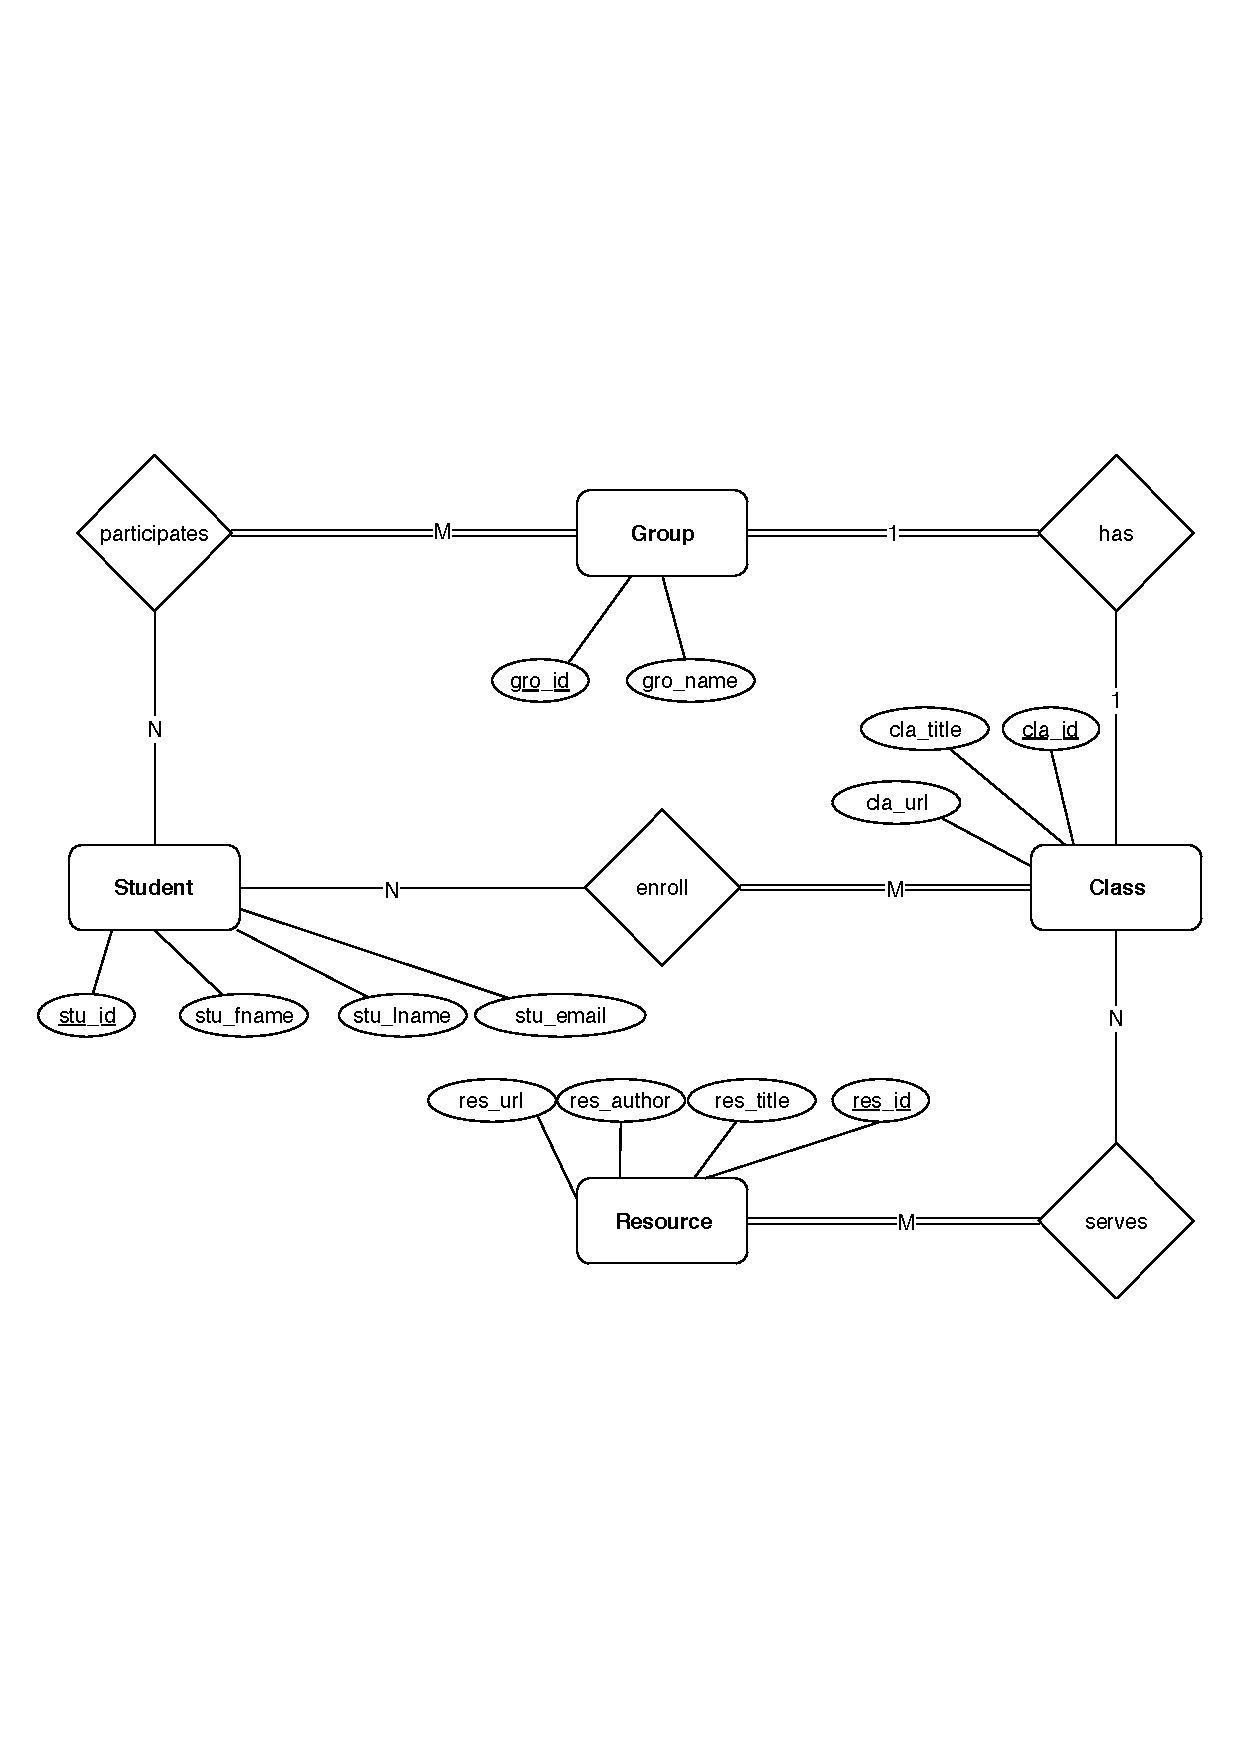
\includepdf[pages={1}]{DB_ERD.pdf}
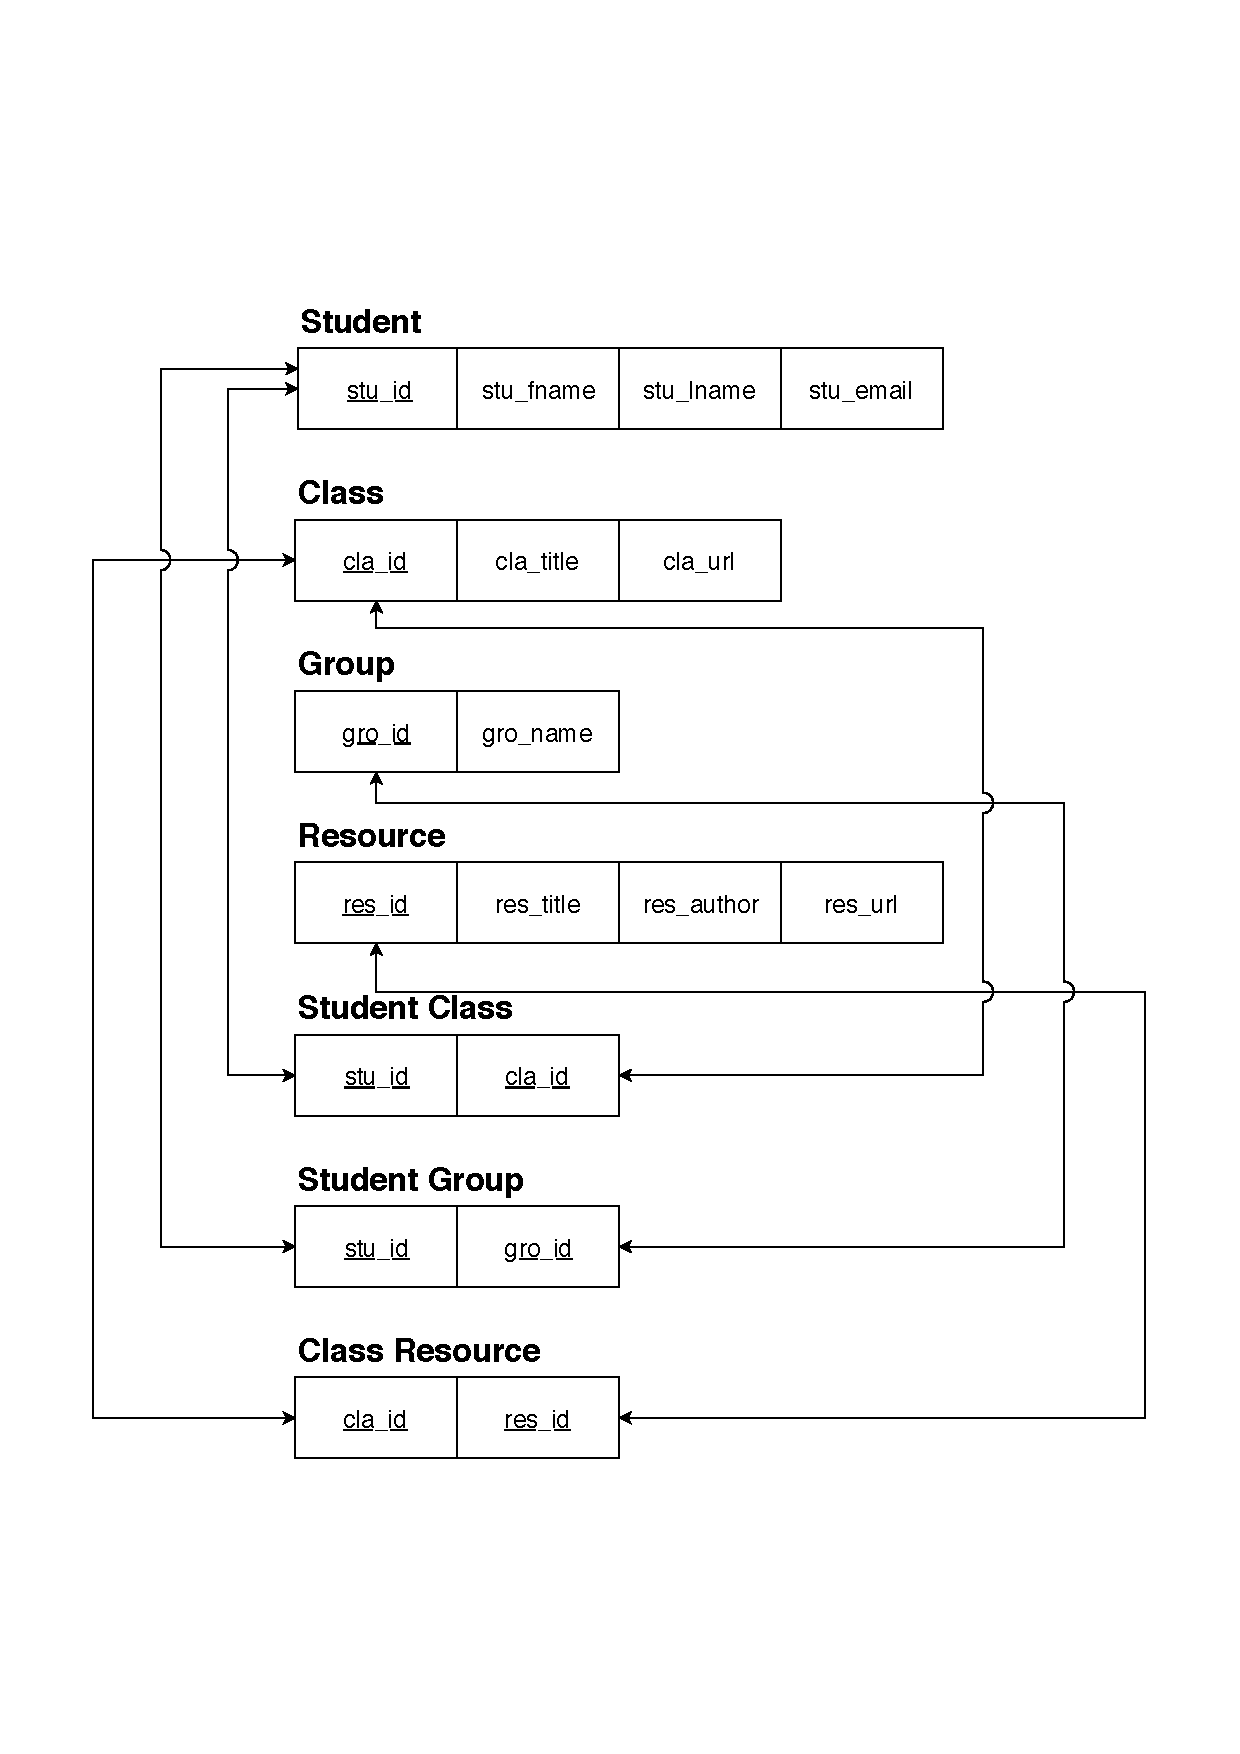
\includepdf[pages={1}]{DB_Schema.pdf}



\end{document}